\chapter{Weak and Strong Interactions}

\begin{center}
\textbf{\begin{huge} October 4, 2011\end{huge}}
\end{center}

Let's begin with:

\begin{align}
P&= \text{ tunneling probability} \sim e^{-(E_G/E)^{1/2}}\\
E_G &= \frac{2 \pi^2 m_r e^4 Z_1^2 Z_2^2}{\hbar^2}\\
&\sim 1 \text{ MeV} Z_1Z_2\frac{m_r}{m_p}\\
\frac{E_G}{E} &\sim \lp \frac{r_c}{\lambda} \rp^2\\
\Aboxed{\sigma(E) &= \frac{S(E)}{E} e^{-(E_G/E)^{1/2}}}~,\text{ cross section for nuclear reactions,}
\end{align}

where $S(E)$ is the nuclear physics part of the cross-section. $\sigma(E)$ is typically in units of barns, where 1 barn = $10^{-24}$ cm. 

A weak interaction has a cross section about $\sim 20$ orders of magnitude less than the strong interaction, although the S-factor is much larger. For example:

\begin{align}
S &\sim 10^{-20} \text{ barn keV}\\
\sigma &\sim 10^{-20} \text{ barn} \sim 10^{-40} \text{ cm}^{2}
\end{align}
 
\section{Particle Interaction}

Let's imagine particles of type 1 interacting with particles of type 2.\\
The $l$ for particle 2: $l_{2} = \frac{1}{n_{1}\sigma}$ and the time between reactions = $\tau_{2} = \frac{l_{2}}{v}=\frac{1}{n_{1}\sigma v}$. The rate of reactions is the number of reactions for particles 1 and 2 per unit volume per unit time.

\begin{align}
\Aboxed{r_{12} &= \frac{n_{2}}{\tau_{2}} = n_{1}n_{2}\sigma v}\\
r_{12} &= n_{1}n_{2}\underbrace{\langle \sigma(E)v\rangle }_{\text{average over MBD}}\\
\langle \sigma(E)v\rangle &= \int d^3 \vec{v} \textrm{prob}(v)\sigma(E)v\\
\Aboxed{&=\underbrace{4 \pi v^{2} dv}_{\textrm{v-space volume}}  v\sigma \underbrace{\lp \frac{m_{r}}{2 \pi kT} \rp^{3/2} e^{-\frac{m_{r}v^{2}}{2kT}}}_{\textrm{Boltzmann probability}}}
\end{align}

\begin{align}
E=\half m_{r}v^{2}\ra dE=m_{r}vdv\\
d^{3}v = 4 \pi v^{2}dv = \frac{8 \pi E}{m_{r}}\frac{dE}{m_{r}v}
\end{align}

Substituting $4 \pi v^{2}dv$:

\begin{align}
\boxed{\langle \sigma v\rangle  = \lp \frac{2}{kT} \rp^{{3/2}} \frac{1}{\sqrt{\pi m_{r}}} \int  E_{\sigma}(E)E^{-E/kT}dE}
\end{align}

\begin{align}
\langle \sigma v\rangle = \lp \frac{2}{kT} \rp^{{3/2}} \frac{1}{\sqrt{\pi m_{r}}} \int S(E) \underbrace{e^{-(E_{0}/E)^{1/2} -E/kT}}_{\textrm{see Fig. \ref{fig:2}}}\\
f(E) =\lp  \frac{E_{G}}{E} \rp^{{1/2}} + \frac{E}{kT}
\end{align}

\begin{figure}[!h]
\centering
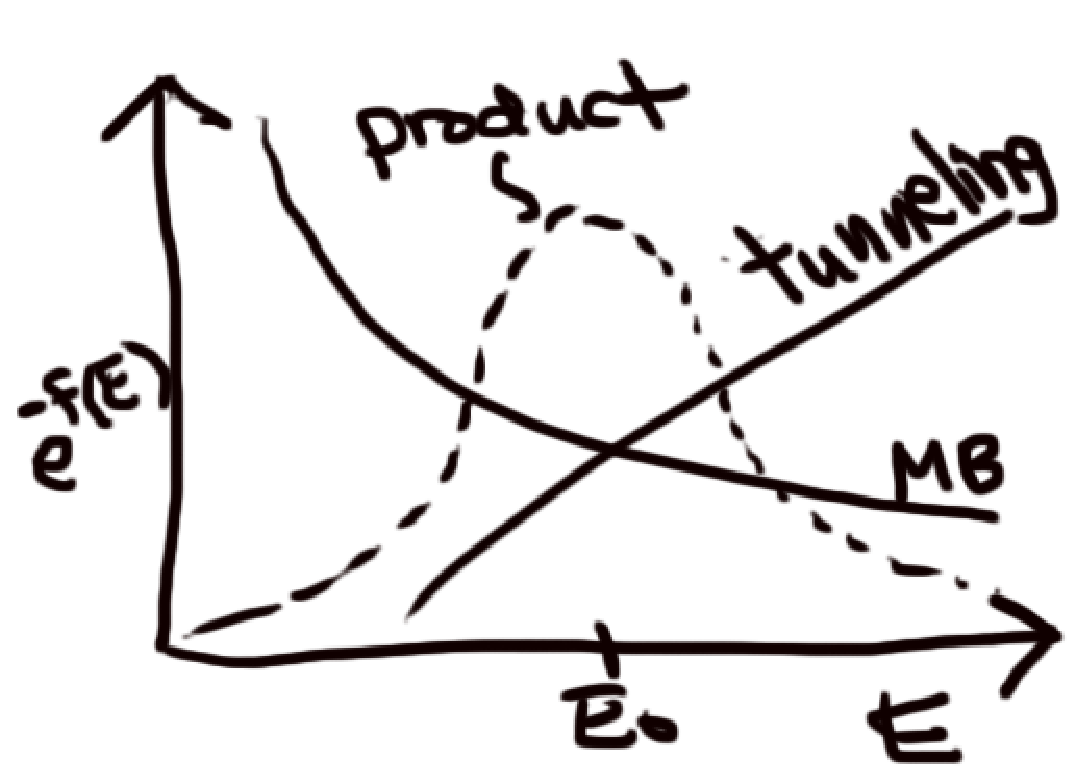
\includegraphics[width=\textwidth/2]{images/fig2.eps}
\label{fig:2}
\caption{}
\end{figure}

Assume $S(E)$ is slowly varying compared to the exponential so that:

\begin{align}
\langle \sigma v\rangle = \lp \frac{2}{kT} \rp^{3/2} \frac{1}{\sqrt{\pi m_{r}}} SI~,I = \int e^{-f(E)}dE~.
\end{align}

$E_{0}$ is the place where $\frac{\delta f}{\delta E} = 0$ i.e., the most probably reaction energy. 

\begin{align}
E_{0} &= \lp \half E_{G}^{1/2}kT\rp^{2/3}~,\textrm{ energy of particles that dominate reactions}\\
E_{0} &\approx (5.7 \textrm{ keV} )Z_{1}^{2/3}Z_{2}^{2/3}T_{7}^{2/3} \lp \frac{m_{r}}{m_{p}} \rp^{1/3}~,T_{7} = T/10^{7}\textrm{K}
\end{align}

At $10^{7}$ K, this roughly corresponds to an energy of 0.87 keV. For the pp chain,

\begin{align}
\underbrace{p + p \ra ...}_{\textrm{at $T \sim 10^{7}$ K}} ~E_{0} \sim 6 \textrm{ keV} \sim 6kT\\
E_{G} \sim 500 \textrm{ keV}~,kT < E_{0} \ll E_{G}\\
S \approx S(E_{0})
\end{align}

We do a Taylor expansion of $f(E)$ to get:

\begin{align}
f(E) &= f(E_{0}) + f' (E_{0})(E - E_{0}) + \half f'' (E_{0})(E-E_{0})^{2}+...\\
I &= e^{-f(E_{0})} \int_{0}^{\infty}e^{-\frac{1}{2} f''(E_{0})(E-E_{0})^{2}}dE\\
f''(E_{0}) &= \frac{3}{4}\frac{E_{G}^{1/2}}{E_{0}^{5/2}} \approx \frac{e^{-f(E_{0})} \sqrt{2\pi}	}{\sqrt{f''(E_{0}}}\\
\underbrace{\langle \sigma v\rangle}_{\textrm{function of $Z_{1},Z_{2},m_{r},T$}} &= \lp \frac{2}{kT}\rp^{3/2}\frac{1}{\sqrt{\pi m_{r}}} S(E_{0})I\\
\Aboxed{\langle \sigma \rangle > &= 2.6 S(E_{0}) \frac{E_{G}^{1/6}}{(kT)^{2/3}\sqrt{m_{r}}} e^{-3(E_{G}/4kT)^{1/3}}}
\end{align}

\section{Energy Generation}

Now, we go back and recall that $r_{12} = n_{1}n_{2}\langle \sigma v\rangle  = $ \# of reactions/vol/time. $Q$ = energy produced by a given reaction.

\begin{align}
\epsilon &= \textrm{erg/s/g generated by reaction } 1 + 2 \ra\\
&= \frac{r_{12}Q}{\rho} = \frac{n_{1}n_{2}\langle \sigma v\rangle Q}{\rho}~,n_{1}=X_{1} \frac{\rho}{m_{1}}
\end{align}

where $X_{1}$ is the fraction of mass in particles of type 1. Now we can write:

\begin{align}
\Aboxed{\epsilon_{12} &= \frac{2.6QS(E_{0})X_{1}X_{2}}{m_{1}m_{2}\sqrt{m_{r}} (kT)^{2/3}} \rho E_{0}^{1/6} e^{-3(E_{G}/4kT)^{1/3}}}
\end{align}

This is a good form because it is not reaction specific. 

\begin{align}
\epsilon &\pt \frac{\rho}{T^{2/3}}e^{-3(E_{G}/4kT)^{1/3}}\\
r &\pt n^{2}\\
\epsilon &\pt \frac{r}{\rho} \pt \rho\\
\Aboxed{\epsilon &\pt \rho^{\alpha}T^{\beta}}~,\alpha=1\textrm{ for a two-body reaction}\\
\ln \epsilon &= \beta \ln T + ...\\
\beta &= \frac{\delta \ln \epsilon}{\delta \ln T} \ra \boxed{ \beta = -\frac{2}{3} + \lp \frac{E_{G}}{4kT} \rp^{1/3}}
\end{align}

\begin{align}
p + p\ra ...~,\textrm{kT}\approx 1\textrm{ keV}\\
E_{G} = 500 \textrm{ keV}~,\beta \approx 4.3\\
\epsilon \pt \rho T^{4.3} \textrm{ near } kT \approx 1\textrm{ keV}
\end{align}

At the center of our sun, $T \sim 10^{7}$ K, $kT=1$ keV, and $\langle \rho\rangle \sim$1 g/cm$^{3}$.

\begin{align}
p + p \ra ... ~,\textrm{ first thing to fuse is the low charge stuff}
\end{align}

For strong interactions, $S \sim $ keV barn $\sim 10^{-33}$ cm$^{2}$ erg. The binding energy per particle released ($Q$) is about 10 MeV. 

\begin{align}
\epsilon \sim 10^{20}\textrm{ ergs/s/g}\\
L = \int \epsilon dM \sim \epsilon M \sim 10^{54}\textrm{ ergs/s } \sim 10^{20} L_{\odot}
\end{align}

We're 20 orders of magnitude off... let's use the weak interaction instead of the strong. 